% !TEX root = ./Masterdatei.tex

\section{Beschreibung}
\subsection{Vision}

Nachrichten, Social Media und Katzenvideos bombardieren uns mit Informationen ohne Ende -
mit negativen Auswirkungen auf Konzentration und Kurzzeitgedächtnis.
Wer dem entgehen möchte, muss seinen Kopf mit regelmäßigem Training auf Trab halten.
Genau dafür ist diese App gedacht.

\enquote{Gedächtnistraining mit n-back} implementiert eine Gedächtnisübung namens
\enquote{n-back-Test}, welche in einem Paper aus dem Jahre 1958 erdacht wurde.
Die tägliche Nutzung der App soll dabei helfen, Kurzzeitgedächtnis und
Konzentrationsfähigkeit des Nutzers zu steigern. Statistiken über die tägliche Nutzung,
darunter Highscores und Diagramme, legen dem Nutzer seine Fortschritte dar und bieten
eine Motivation zur Weiternutzung der App.

\subsection{Zielgruppe}

Die App ist auf jeden ausgerichtet, der sein Gedächtnis trainieren möchte:
Darunter sind Schüler, Studenten, Erwachsene und insbesondere ältere Menschen.
\enquote{Gedächtnis\-training mit n-back} eignet sich auch für Personen, die wenig Zeit haben,
denn wenige Minuten täglichen Trainings sollen sichtbare Ergebnisse liefern.

\subsection{Die App}

Allgemein läuft ein n-back-Test folgendermaßen ab:
Einer Testperson wird nacheinander eine Menge von Reizen gegeben (Zahlen, Farben, Geräusche, ...).
Die Aufgabe besteht darin, sich jederzeit eine bestimmte Anzahl (= n) vergangener Reize zu merken
und abrufen zu können.
Konkret soll in dieser App ein arithmetischer n-back-Test implementiert werden.
Dabei wird dem Nutzer nacheinander ein simpler arithmetischer Ausdruck (deren Lösung einstellig ist) vorgegeben.
Das Ziel ist jeweils das Ergebnis anzugeben, dass zu dem Ausdruck n Stellen zuvor gehört.
(Beispielsweise wird bei n=1 das Ergebnis des vorherigen Ausdrucks erwartet, bei n=2 das Ergebnis des vorvorletzten Ausdrucks etc.)


\section{Entwurf}
Im folgenden Abschnitt werden die Funktionen der App beschrieben und im Anschluss mittels Illustrationen veranschaulicht.

\subsection{Funktionsbeschreibung}
\subsubsection{Hauptmenü}

Das Hauptmenü ist der Screen, der beim Starten der App immer als erstes erscheint.
Es enthält Einträge, über die man auf die anderen Funktionen der App zugreifen kann.
Dazu gehören:
\begin{itemize}[itemsep=0pt]
  \item Das Starten der Übung
  \item Das Konfigurieren der Übungsparameter
  \item Das Einsehen der Statistiken
\end{itemize}

\noindent (Siehe Abb \ref{menu} für eine Skizze des Hauptmenüs)

\subsubsection{Übung starten}

Eine Übung besteht aus einer Menge an Runden.
In jeder Runde wird dem Nutzer ein Ausdruck gezeigt, woraufhin er
eine Zahl auswählt. Ob diese Eingabe korrekt ist (d.h. zu dem Ausdruck n Stellen zuvor passt\footnote{Für die ersten n Runden wird keine Eingabe erwartet, hier soll nach 2-3 Sekunden die nächste Runde von Selbst starten})
soll dem Nutzer farblich vermittelt werden (z.B. korrekt = Eingabe grün färben; falsch = Eingabe rot, korrekte Antwort blau färben).
Nach der Eingabe startet die nächste Runde mit dem Anzeigen eines neuen Ausdrucks.
Wann die Übung endet hängt von den gewählten Übungsparametern (siehe \ref{konfig}) ab:
\begin{itemize}[itemsep=0pt]
  \item Nach einer bestimmten Menge an Runden
  \item Nach der nächsten Runde ab Ablauf eines bestimmten Zeitlimits
\end{itemize}
Zusammenfassend enthält der Bildschirm während einer Übung folgende Elemente:
\begin{itemize}[itemsep=0pt]
  \item Den aktuellen Ausdruck
  \item Ein Nummernfeld zur Eingabe der Antwort
  \item Die aktuelle Rundenzahl
  \item Die Endbedingung der Übung: Maximale Rundenzahl oder verbleibende Zeit
\end{itemize}
Ist die Übung beendet, wird der Ergebnisbildschirm angezeigt, dieser enthält
folgende Informationen:
\begin{itemize}[itemsep=0pt]
  \item Den Parameter n
  \item Die Anzahl der korrekten Eingaben
  \item Die Anzahl aller Eingaben
  \item Die Trefferquote (\#korrekt / \#gesamt)
  \item Die erzielte Punktzahl \footnote{Für die Berechnung der Punktzahl, siehe \ref{score}}
  \item Die höchste heute erzielte Punktzahl
  \item Die höchste jemals erzielte Punktzahl
\end{itemize}
Für jede Übung werden die Punktzahl, Parameter n und das Datum lokal gespeichert,
um Statistiken erstellen zu können. (siehe \ref{statistiken})

Aus dem Ergebnisbildschirm führen den Nutzer 2 Buttons: Einer soll ihn zurück in das Hauptmenü bringen,
der andere startet eine neue Übung mit den selben Parametern.

\noindent Abb. \ref{ablauf} stellt einen möglichen Ablauf für eine Übung mit
n=1 dar.

\subsubsection{Konfigurationsmenü}
\label{konfig}
In diesem Menü sollen die Übungsparameter geändert werden können.
Zu jedem Parameter soll es einen Eintrag bestehend aus dem Namen und dem aktuellen Wert geben.
Berührung eines Eintrags öffnet ein zum Parametertyp passendes Eingabewidget, Auswahl eines Wertes aktualisiert den
im Eintrag angezeigten Wert.
Zusätzlich sollen dem Nutzer 3 Buttons (etwa in einer Appbar) zur Verfügung stehen:
\begin{itemize}[itemsep=0pt]
  \item Änderungen übernehmen
  \item Änderungen verwerfen
  \item Defaultwerte wiederherstellen
\end{itemize}
Jeder dieser Buttons soll den Nutzer erst mit einem Popup fragen, ob er die Aktion
wirklich durchführen will, bei Bestätigung dann die Aktion ausführen und den
Nutzer zurück in das Hauptmenü bringen.

\begin{samepage}
\noindent Mindestens sollen folgende Parameter existieren:
\begin{itemize}[itemsep=0pt]
  \item n (\texttt{type = integer, default = 1})\\
  Schwierigkeitsgrad der Übung; Gibt an, zu welchem Ausdruck (relativ zum aktuellen Ausdruck) die Lösung erwartet wird.
  \item Übungsende (\texttt{type = Enum [ZEIT, ANZAHL], default = ANZAHL})\\
  Gibt an, ob das Ende der Übung anhand eines Zeitlimits (ZEIT) oder anhand der Anzahl der Runden (ANZAHL) feststeht.
  \item Zeitlimit (\texttt{type = [integer, integer], default = [3, 0]})\\
  Anzahl der Minuten und Sekunden, nach deren Ablauf die Übung endet (wenn als Übungsende ZEIT gewählt wurde).
  \item Rundenlimit (\texttt{type = integer, default = 20})\\
  Anzahl der Runden, bevor die Übung endet (wenn als Übungsende ANZAHL gewählt wurde).
\end{itemize}
\end{samepage}

\subsubsection{Statistiken}\label{statistiken}
Zur Motivation soll der Nutzer hier Statistiken über abgeschlossene Übungen abrufen können.
Um Übungen mit unterschiedlichen Parametern vergleichen zu können, soll zu jeder Übung
eine Punktzahl errechnet werden.
Eine mögliche Punktzahlfunktion könnte so aussehen:\label{score}
$$
  \textit{Score} = (\textit{\#korrekt} - \lceil 0.5 * \textit{\#falsch} \rceil) * 10^n
$$

\noindent Das Statistiken-Menü  soll 2 Unterfunktionen bieten, die im Folgenden
beschrieben werden.

\paragraph{Übungsliste}
Hier werden alle abgeschlossenen Übung untereinander aufgelistet.
Jeder Eintrag enthält Datum, n und Punktzahl der Übung.
Sortiert soll die Liste anfangs aufsteigend nach Datum sein,
über einen Button in der Appbar soll der Nutzer zwischen Sortierung nach Datum und nach Punktzahl wechseln können.

\paragraph{Diagramme}
Hier soll der Nutzer seine Leistung in einem von ihm gewählten Zeitraum in Form eines Diagrammes
betrachten können.

\begin{samepage}
\noindent Der Nutzer soll 3 Auswahlmöglichkeiten für den Zeitraum haben:
\begin{itemize}[itemsep=0pt]
  \item aktuelle Woche
  \item aktueller Monat
  \item aktuelles Jahr
\end{itemize}
\end{samepage}
Nach Auswahl eines Zeitraumes soll ein Diagramm generiert werden:
\begin{itemize}[itemsep=0pt]
  \item Die x-Achse sei die Zeit
  \item Die y-Achse sei der Punktestand
  \item Jede Übung, die im gewählten Zeitraum stattfand, bildet einen Punkt mit x = Datum, y = Punktzahl
\end{itemize}
Die Eingabe für den Zeitraum soll sich auf dem selben Screen befinden wie das Diagramm. Standardmäßig wird beim Öffnen
des Diagramm-Screens der Zeitraum 'Woche' gewählt und das entsprechende Diagramm für die aktuelle Woche angezeigt.
Durch Auswahl eines anderen Zeitraums wird sofort ein neues Diagramm generiert.
\newpage

\subsection{Skizzen}
\begin{figure}[htbp]
\begin{subfigure}{.33\textwidth}
  \centering
  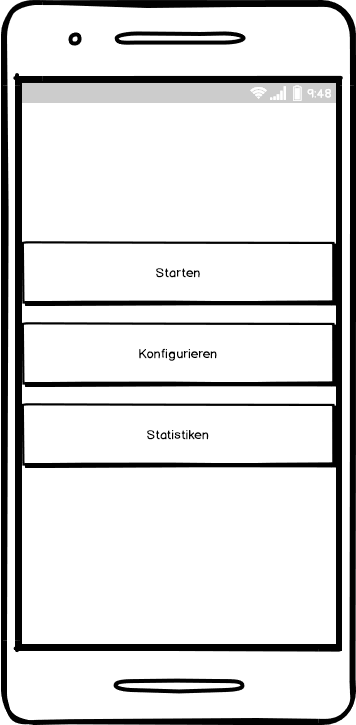
\includegraphics[width=0.7\textwidth]{img/mainmenu}
  \caption{Das Hauptmenü}
  \label{menu}
\end{subfigure}
\begin{subfigure}{.33\textwidth}
  \centering
  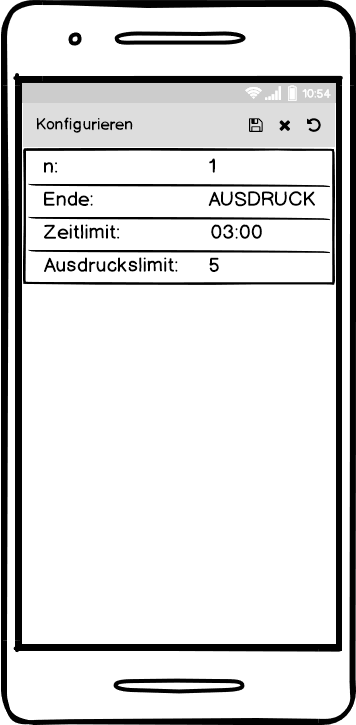
\includegraphics[width=0.7\textwidth]{img/konfig_menu.png}
  \caption{Das Konfigurationsmenü}
  \label{config}
\end{subfigure}
\begin{subfigure}{.33\textwidth}
  \centering
  \includegraphics[width=0.7\textwidth]{img/statmenu.png}
  \caption{Das Statistikenmenü}
\end{subfigure}
\begin{subfigure}{.33\textwidth}
  \centering
  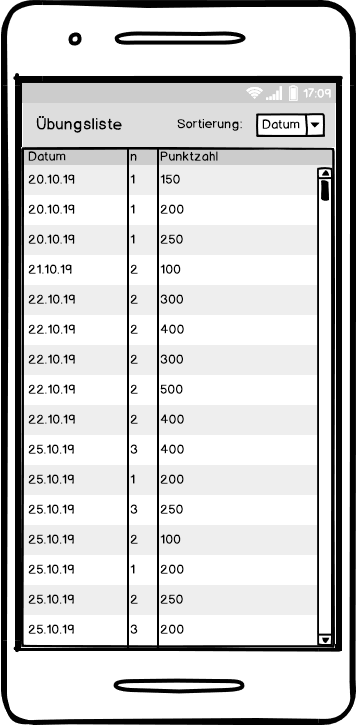
\includegraphics[width=0.7\textwidth]{img/list.png}
  \caption{Die Übungsliste}
\end{subfigure}
\begin{subfigure}{.33\textwidth}
  \centering
  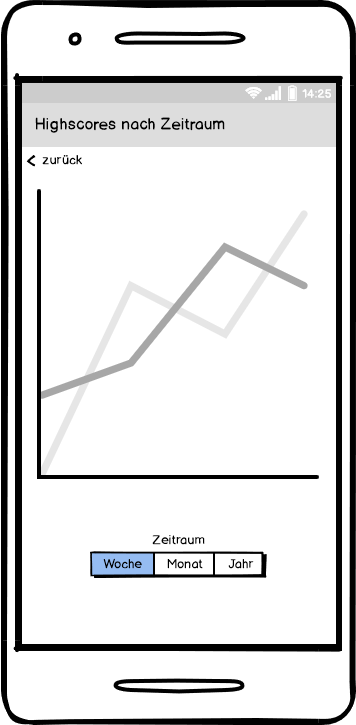
\includegraphics[width=0.7\textwidth]{img/stat_daily.png}
  \caption{Der Diagrammbildschirm}
\end{subfigure}
\end{figure}

\begin{figure}[htbp]
\centering
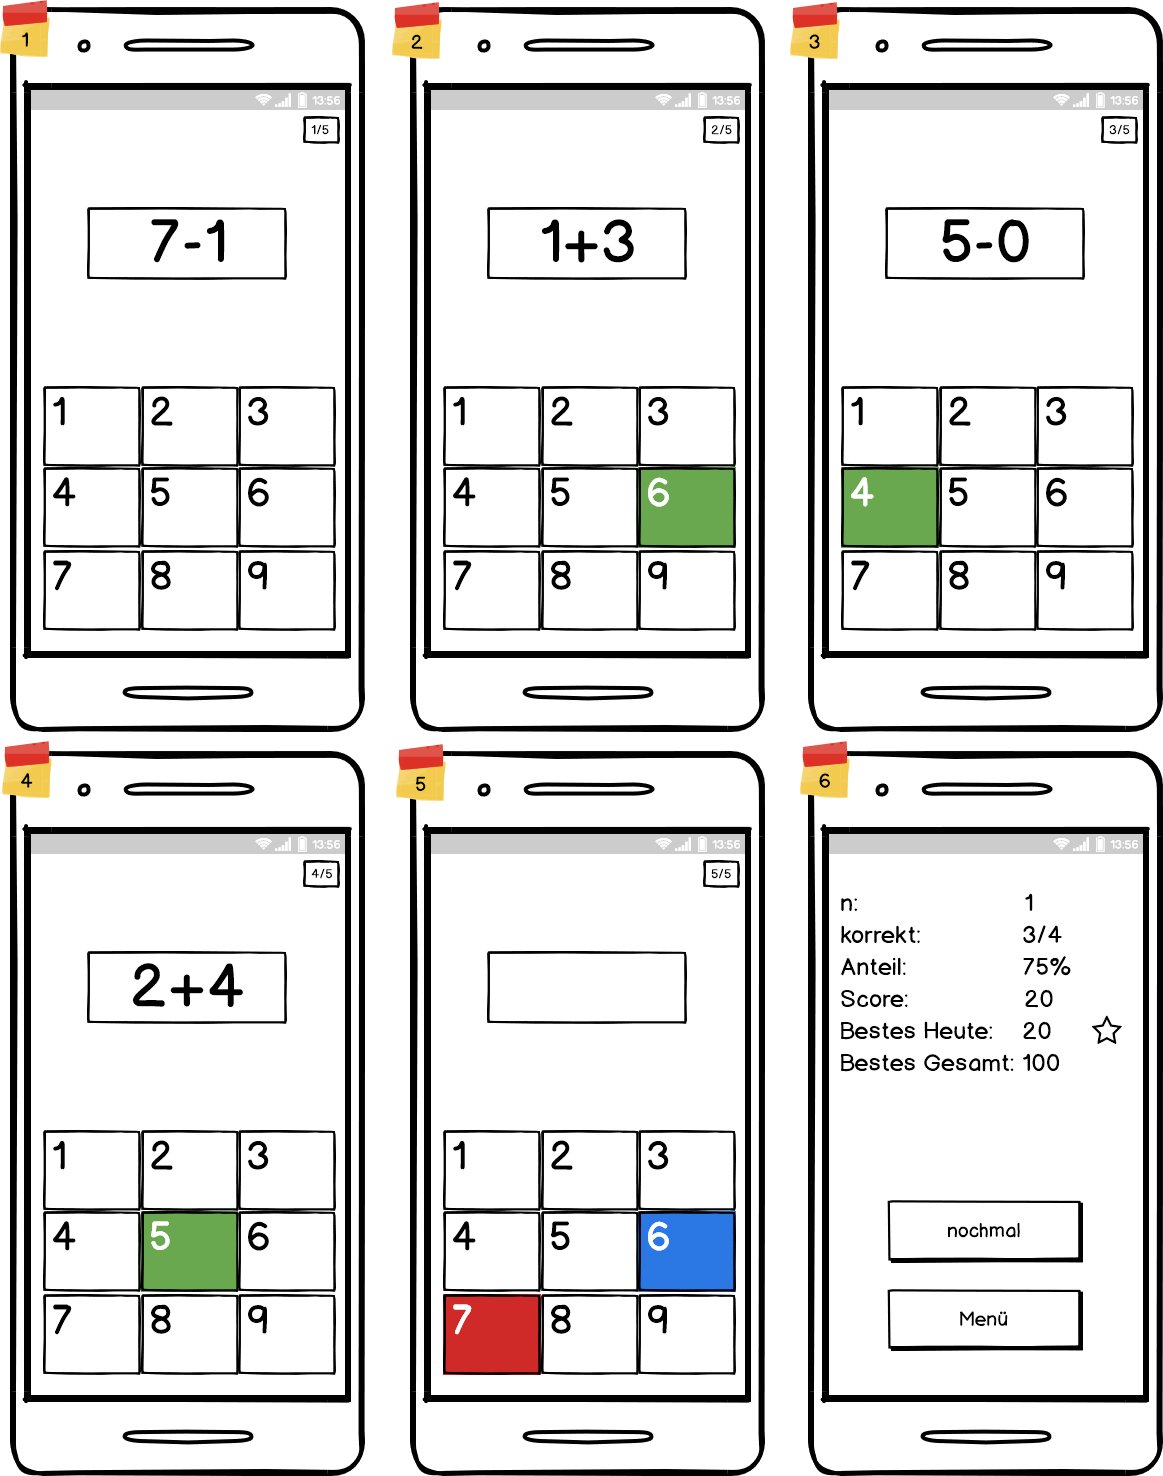
\includegraphics[width=1\textwidth]{img/ubungFull.png}
\caption{Ablauf einer Übung mit n=1}
\label{ablauf}
\end{figure}

\begin{figure}[htbp]
\centering
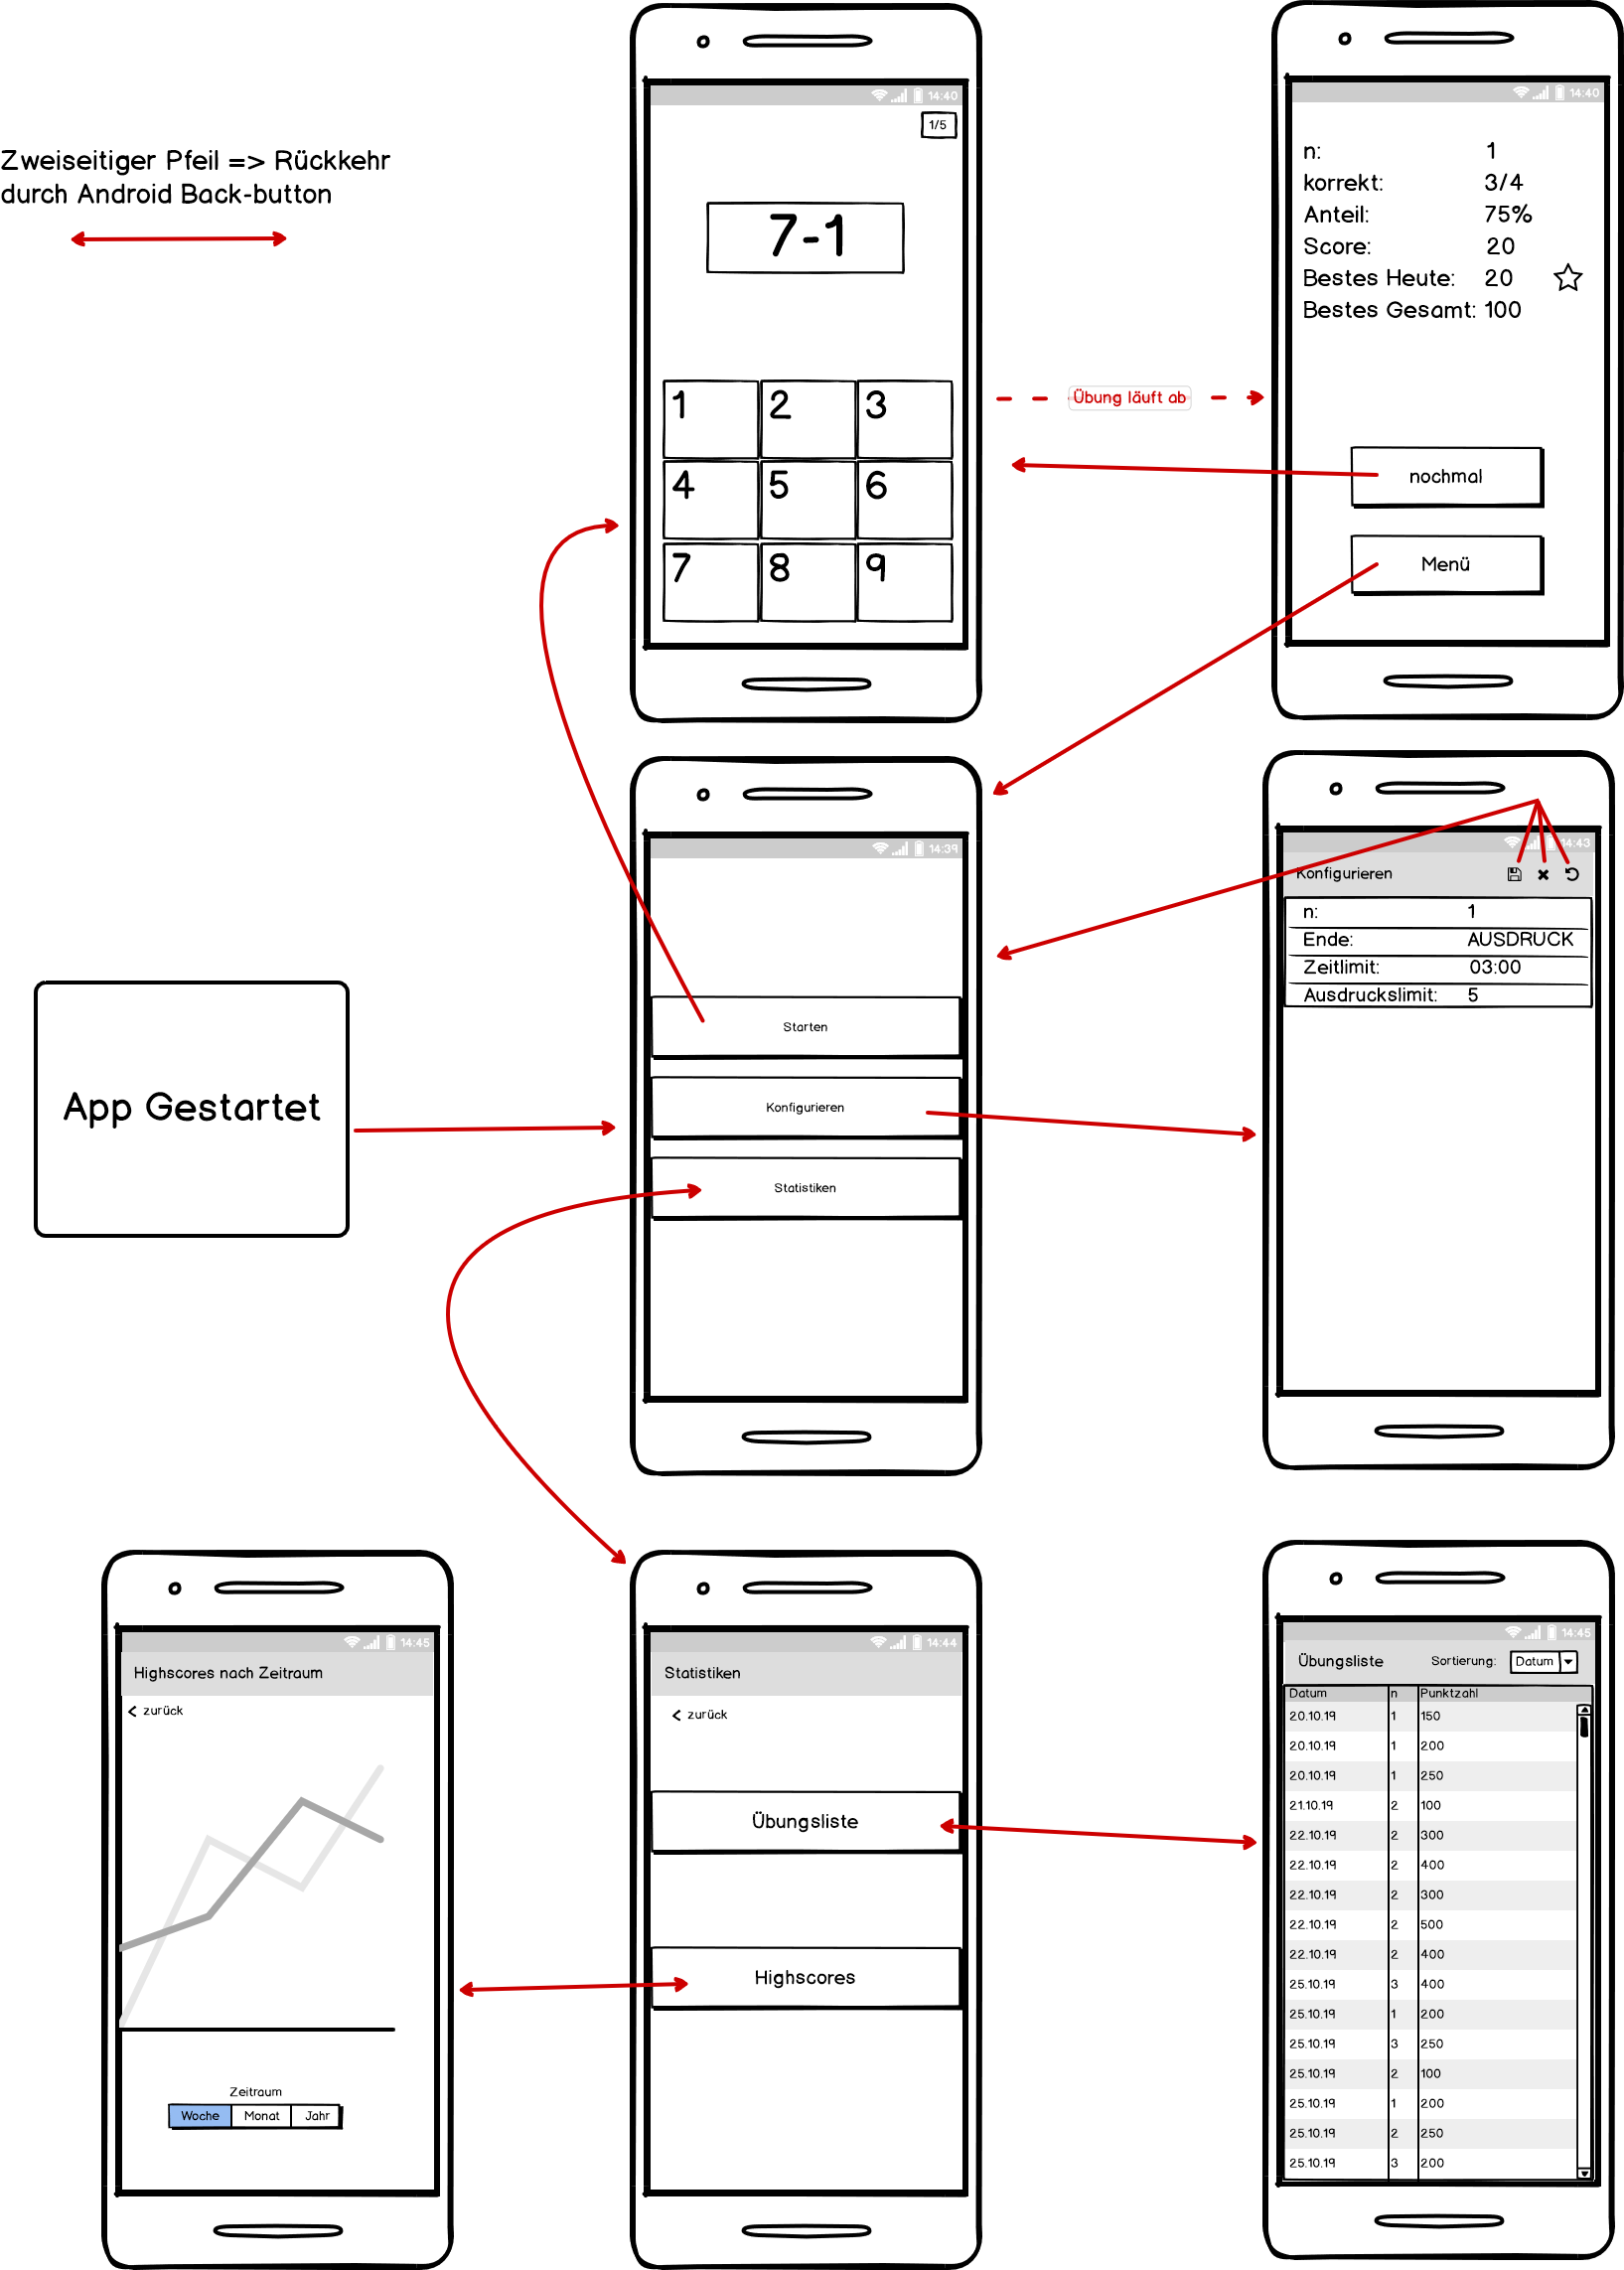
\includegraphics[width=0.98\textwidth]{img/Ablauf}
\caption{Übersicht über den Ablauf der Screens}
\end{figure}

\newpage
\subsection{Optionale Funktion: Musikalische Untermalung}
\begin{addmargin}[25pt]{0pt}
\textit{Die in diesem Abschnitt beschriebene Funktion kann implementiert werden, ist aber nicht zwingend erforderlich.
  Eine Implementierung muss sich auch nicht exakt an die Beschreibung in diesem Kapitel halten.
}
\end{addmargin}
Der Nutzer kann sich eine Musikdatei aussuchen, diese wird dann während der Übung abgespielt.
Folgende zusätliche Parameter werden hierzu im Konfigurationsmenü (Abschnitt \ref{konfig}) angeboten:
\begin{itemize}[itemsep=0pt]
  \item Musikdatei (\texttt{type = string, default = 'none'})\newline
  Titel einer Musikdatei auf dem Gerät
  \item Abspielart (\texttt{type = Enum [NOTENWEISE, STANDARD], default = STANDARD})\newline
  Gibt an, wie das Musikstück wiedergegeben wird
\end{itemize}
Ist eine Musikdatei gewählt (d.h. Parameter 'Musikdatei' ungleich 'none') wird während der Übung das gewählte
Stück auf einer von zwei möglichen Arten wiedergegeben, abhängig vom Parameter 'Abspielart':
\begin{itemize}[itemsep=0pt]
  \item \texttt{'Abspielart' = 'NOTENWEISE'}:\newline
  Zu jeder richtigen Antwort des Nutzers wird ein Ton des Stücks abgespielt.
  Bei einer falschen Antwort wird entweder ein Ton übersprungen, oder ein Fehlerton abgespielt.
  \item \texttt{'Abspielart' = 'Standard'}:\newline
  Zu Beginn der Übung wird die Wiedergabe des Musikstücks gestartet.
\end{itemize}
Berührt der Nutzer den Eintrag 'Musikdatei' im Konfigurationsmenü wird eine Liste verfügbarer Musikdateien angezeigt.
Diese kann auf eine (oder Beide) von zwei Arten befüllt werden:
\begin{itemize}[itemsep=0pt]
  \item Das Gerät wird nach Musikdateien durchsucht
  \item Die App stellt Musikdateien bereit
    \footnote{
      Hierbei muss unbedingt auf die jeweiligen Urheberbedingungen der Musikstücke geachtet werden. Eventuell muss
      der Urheber jedes verwendeten Musikstücks auf einem seperatem Screen genannt werden,
      zu dem man beispielsweise aus dem Hauptmenü gelangt.
    }
\end{itemize}

%%% Matthias Ramsauer

\subsection{Releaseplanung}
\begin{table}[H]
\centering
\begin{tabular}{>{\centering\arraybackslash}m{0.1\textwidth} | m{0.9\textwidth} }
  \textbf{Release} & \textbf{Funktion mit den wesentlichen Tätigkeiten} \\
  \hline
  v0.0 & \begin{itemize}[leftmargin=*,itemsep=0pt]
    \item Initalisierung Android Projekt
    \item Hauptmenü-Activity (Abb~\ref{menu}) Erstellen
  \end{itemize} \\
  \hline
  v0.1 & \begin{itemize}[leftmargin=*,itemsep=0pt]
    \item Einstellungen-Activity (Abb~\ref{config}) Erstellen
    \item Speichern über \texttt{SharedPreferences}
    \item Implementierung der Toolbar
  \end{itemize} \\
  \hline
  v0.2 & \begin{itemize}[leftmargin=*,itemsep=0pt]
    \item Implementierung der \texttt{GameActivity} (Abb~\ref{ablauf})
    \item Implementierung der \texttt{ScoreActivity}
    \item Implementierung der \enquote{ANZAHL} Abschlussbedingung
      (Sec~\ref{konfig})
    \item Erstellen der Github-Repository
  \end{itemize} \\
  \hline
  v0.3 & \begin{itemize}[leftmargin=*,itemsep=0pt]
    \item Implementierung der \enquote{ZEIT} Abschlussbedingung
      (Sec~\ref{ablauf})
  \end{itemize} \\
  \hline
  v0.4 & \begin{itemize}[leftmargin=*,itemsep=0pt]
    \item Implementierung der Statistiken
    \item Speicherung der Daten über SQLite
  \end{itemize} \\
  \hline
  v0.5 & \begin{itemize}[leftmargin=*,itemsep=0pt]
    \item Bessere Beschreibungen in den Einstellungen
    \item Refactoring
  \end{itemize} \\
  \hline
  v0.6 & \begin{itemize}[leftmargin=*,itemsep=0pt]
    \item Tests erstellen und Bugfixen
  \end{itemize} \\
  \hline
  v1.0 & \begin{itemize}[leftmargin=*,itemsep=0pt]
    \item Release vorbereiten
  \end{itemize} \\
  \hline
  v1.1 & \begin{itemize}[leftmargin=*,itemsep=0pt]
    \item Optionale Features implementieren
  \end{itemize} \\
\end{tabular}
\end{table}
